%%%%%%%%%%%%%%%%%%%%%%%%%%%%%%%%%%%%%%%%%%%%%%%%%%%%%%%%%
 % Zawartość tego projektu jest niemodyfikowalna. 
 % Jeżeli chcesz wprowadzić w nim zmiany, to musisz utworzyć jego kopię — patrz https://www.overleaf.com/learn/how-to/Copying_a_project
 %%%%%%%%%%%%%%%%%%%%%%%%%%%%%%%%%%%%%%%%%%%%%%%%%%%%%%%%%
 %
 %	Name			:: 	The official template for the typesetting of diploma theses at the Faculty of Computer Science of AGH University of Krakow
 %	Author			:: 	Stanisław Polak (polak[aT]icsr[DoT]agh[DoT]edu[DoT]pl)
 %	Created			::	2024-02-14
 %	Modified	    ::	2024-03-04
 %	Version			:: 	1.3.1
 %	Email			:: 	polak[aT]icsr[DoT]agh[DoT]edu[DoT]pl
 %	Website			:: 	http://www.icsr.agh.edu.pl/~polak/
 %   Youtube         ::  https://www.youtube.com/user/spolak69
 %   Github          ::  https://github.com/polaksta
 %	License			:: 	This work may be distributed and/or modified under the
 %                       conditions of the LaTeX Project Public License, either version 1.3
 %                       of this license or (at your option) any later version.
 %                       The latest version of this license is in
 %                       http://www.latex-project.org/lppl.txt
 %                       and version 1.3 or later is part of all distributions of LaTeX
 %                       version 2005/12/01 or later.
 %
 %	Description		::	This document is a demonstration of the template
 %
 %%%%%%%%%%%%%%%%%%%%%%%%%%%%%%%%%%%%%%%%%%%%%%%%%%%%%%%%%
 % Niniejszy dokument — szkielet pracy dyplomowej — prezentuje przykłady użycia klasy 'agh-wi' oraz pakietów tradycyjnie używanych w pracach
 % dyplomowych z informatyki. Dla kilku z nich, wartości początkowe parametrów konfiguracyjnych są zdefiniowane 
 % w klasie  — wartości te uwzględniają uwagi osób prowadzących przedmiot "Pracownia Dyplomowa". 
 % Oczywiście możesz używać dowolnych pakietów, niekoniecznie tych, które są pokazane w tym dokumencie
 %%%%%%%%%%%%%%%%%%%%%%%%%%%%%%%%%%%%%%%%%%%%%%%%%%%%%%%%%
 % Poniższe uwagi NIE DOTYCZĄ Overleaf-a
 %%%%%%%%%%%%%%%%%%%%%%%%%%%%%%%%%%%%%%%%%%%%%%%%%%%%%%%%%
 % W tej przykładowej pracy dyplomowej użyto, między innymi, pakietów:
 %   - "minted", co oznacza, że musisz uruchomić kompilator z opcją '-shell-escape'
 %   - "biblatex", co oznacza, że po kompilacji (dokumentu) musisz, jeszcze, wygenerować plik '.bbl'
 %   - "nomencl", co oznacza, że za pomocą komendy 'makeindex' musisz wygenerować wykaz symboli
 %
 % Tak więc, w celu wygenerowania wynikowego dokumentu PDF, musisz wykonać następujące komendy:
 %       pdflatex -shell-escape example
 %       biber example
 %       makeindex example.nlo  -s nomencl.ist -o example.nls
 %       pdflatex -shell-escape example
 %       pdflatex -shell-escape example
 %
 % Dodatkowo musisz mieć zainstalowany program 'pygmentize', który jest częścią pakietu "Pygments" (https://pygments.org/)
 % Ww. programy powinny zainstalować się automatycznie podczas instalacji pakietów LaTeX
 %
 % Jeżeli masz zainstalowany program 'latexmk', to możesz wygenerować dokument PDF następująco:
 %       latexmk example
 %       makeindex example.nlo  -s nomencl.ist -o example.nls
 %       latexmk example
 %
 % Do edycji (oraz komplilacji) dokumentów LaTeX polecam program 'TeXstudio' (https://www.texstudio.org/)
 %
 % Autor: Stanisław Polak <polak[aT]agh[DoT]edu[DoT]pl>
 %%%%%%%%%%%%%%%%%%%%%%%%%%%%%%%%%%%%%%%%%%%%%%%%%%%%%%%%%
 \documentclass[data-science]{agh-wi} % Praca po polsku; na stronie tytułowej, najpierw jest widoczny polskojęzyczny tytuł, a potem angielskojęzyczny.
 % Kierunek 'Informatyka'.
 % Przeznaczona do oglądania przy użyciu przeglądarki PDF.
%%%%%%%%%%%%%%%%%%%%%%%%%%%%%%%%%
% Inne, przykładowe, użycia klasy
%%%%%%%%%%%%%%%%%%%%%%%%%%%%%%%%%
% \documentclass[english]{agh-wi}               % Praca po angielsku; 
                           %     strona tytułowa po polsku, ale najpierw jest widoczny angielskojęzyczny tytuł, a potem polskojęzyczny.  
                           % Kierunek 'Informatyka'.
                           % Przeznaczona do oglądania przy użyciu przeglądarki PDF.
% \documentclass[english, data-science]{agh-wi} % Praca po angielsku; ...
                           % Kierunek 'Informatyka - Data Science'.
                           % Przeznaczona do oglądania przy użyciu przeglądarki PDF.
% \documentclass[print]{agh-wi}                 % Praca po polsku; ...
                           % Kierunek 'Informatyka'.
                           % Przeznaczona do drukowania - każda strona posiada,
                           %    dodatkowy (2cm), margines na oprawę.
%%%%%%%%%%%%%%%%%%%%%%%%%%%%%%%%%%%%%
% Parametry dla strony tytułowej
%%%%%%%%%%%%%%%%%%%%%%%%%%%%%%%%%%%%%
\titlePL{Generacja muzyki przy pomocy dużych modeli językowych}  % Tytuł po polsku
\titleEN{Music generation with Lange Language Models} % Tytuł po angielsku
\author{Filip Ręka}
\supervisor{dr hab. Maciej Smołka prof. AGH}
%%%%%%%%%%%%%%%%%%%%%%%%%%%%%%%%%%%%%
% Pakiety
%%%%%%%%%%%%%%%%%%%%%%%%%%%%%%%%%%%%%
% Podstawowe — na pewno będziesz ich potrzebował(a) w swojej wersji pracy dyplomowej
%%%%%%%%%%%%%%%%%%%%%%%%%%%%%%%%%%%%%
\usepackage{polski} % Obsługa języka polskiego
%%%%%%%%%%%%%%%%%%%%%%%%%%%%%%%%%%%%%
% Dodatkowe — niekoniecznie będziesz ich potrzebował(a) w swojej wersji pracy dyplomowej
%%%%%%%%%%%%%%%%%%%%%%%%%%%%%%%%%%%%%
\usepackage[sorting=none]{biblatex}           % Spis literatury ma być tworzony na podstawie zawartości bibliograficznej bazy danych
\usepackage{amsmath}                          % Dodatkowe środowiska matematyczne
\usepackage{amssymb}                          % Dodatkowe symbole matematyczne
\usepackage[polish, intoc]{nomencl}           % Definiowanie symboli
\usepackage{graphicx}                         % Wstawianie grafik zewnętrznych
\usepackage{xcolor}                           % Kolorowy tekst
\usepackage{tabularx}                         % Rozszerzona wersja środowiska 'tabular'
\usepackage{longtable}                        % Skład "długich" tabel
\usepackage[ruled,linesnumbered]{algorithm2e} % Algorytmy w formie pseudokodu
\usepackage{listings}                         % Formatowanie kodów źródłowych programów
\usepackage[newfloat]{minted}                 % Formatowanie kodów źródłowych programów
\usepackage{hyperref}                         % Obsługa adresów URL — zbędny jeżeli używasz 'biblatex'
\usepackage{csquotes}                         % Polskie cudzysłowy — rekomendowany jeżeli używasz 'biblatex'
\usepackage{tocloft}
\usepackage{lipsum}

% NAJWAŻNIEJSZE POLECENIE
\newcommand{\shrug}[1][]{%
\begin{tikzpicture}[baseline,x=0.8\ht\strutbox,y=0.8\ht\strutbox,line width=0.125ex,#1]
\def\arm{(-2.5,0.95) to (-2,0.95) (-1.9,1) to (-1.5,0) (-1.35,0) to (-0.8,0)};
\draw \arm;
\draw[xscale=-1] \arm;
\def\headpart{(0.6,0) arc[start angle=-40, end angle=40,x radius=0.6,y radius=0.8]};
\draw \headpart;
\draw[xscale=-1] \headpart;
\def\eye{(-0.075,0.15) .. controls (0.02,0) .. (0.075,-0.15)};
\draw[shift={(-0.3,0.8)}] \eye;
\draw[shift={(0,0.85)}] \eye;
% draw mouth
\draw (-0.1,0.2) to [out=15,in=-100] (0.4,0.95); 
\end{tikzpicture}}

%%%%%%%%%%%%%%%%%%%%%%%%%%%%%%%%%%%%
%  % Konfiguracja rysunków TikZ
%%%%%%%%%%%%%%%%%%%%%%%%%%%%%%%%%%%%
\usetikzlibrary{shapes.geometric,arrows.meta} 
\tikzstyle{every picture}+=[remember picture]
\tikzstyle{na} = [baseline=-.5ex]
%%%%%%%%%%%%%%%%%%%%%%%%%%%%%%%%%%%%
% Ładowanie danych bibliograficznych
%%%%%%%%%%%%%%%%%%%%%%%%%%%%%%%%%%%%
\addbibresource{bibliography.bib}
%%%%%%%%%%%%%%%%%%%%%%%%%%%%%%%%%%%%%
% Opcje konfiguracyjne pakietów
%%%%%%%%%%%%%%%%%%%%%%%%%%%%%%%%%%%%%
% Pakiet 'framed'
\definecolor{shadecolor}{gray}{0.9}
% Pakiet 'nomencl'
\makenomenclature % Otwórz plik 'example.nlo'
%%%%%%%%%%%%%%%%%%%%%%%%%%%%%%%%%%%%%
% Definicje komend
%%%%%%%%%%%%%%%%%%%%%%%%%%%%%%%%%%%%%
\newcommand{\alert}[1]{\colorbox{red!50}{#1}}
%%%%%%%%%%%%%%%%%%%%%%%%%%%%%%%%%%%%%
% Twierdzenia i podobne struktury
%%%%%%%%%%%%%%%%%%%%%%%%%%%%%%%%%%%%%
\newtheorem{theorem}{Twierdzenie}
\newtheorem{definition}{Definicja}

%%%%%%%%%%%%%%%%%%%%%%%%%%%%%%%%%%%%%
% Ustawienie licznika do subsubsection
%%%%%%%%%%%%%%%%%%%%%%%%%%%%%%%%%%%%%
\setcounter{secnumdepth}{5}

\newcounter{comment}[chapter]
\newenvironment{comment}[1][]{\begin{shaded}\refstepcounter{comment}
\noindent \textbf{Uwaga~\thechapter.\thecomment. #1} \rmfamily}{\end{shaded}}
%%%%%%%%%%%%%%%%%%%%%%%%%%%%%%%%%%%%%
%%%%%%%%%%%%%%%%%%%%%%%%%%%%%%%%%%%%%
\begin{document}
%%%%%%%%%%%%%%%%%%%%%%%%%%%%%%%%%%%%%
\frontmatter % Część wstępna
%%%%%%%%%%%%%%%%%%%%%%%%%%%%%%%%%%%%%
\maketitle % Dodaj stronę tytułową
%%%%%%%%%%%%%%%%%%%%%%%
% Jeżeli chcesz komuś podziękować, to możesz użyć poniższego kodu
\cleardoublepage
\thispagestyle{empty}
\vspace*{\fill}
\begin{flushright}
    \em
    \begin{minipage}{0.75\textwidth}
        Tutaj możesz umieścić treść podziękowań.
        Tutaj możesz umieścić treść podziękowań.
        Tutaj możesz umieścić treść podziękowań.
        Tutaj możesz umieścić treść podziękowań.
        Tutaj możesz umieścić treść podziękowań.
    \end{minipage}
\end{flushright}
%%%%%%%%%%%%%%%%%%%%%%%
\begin{abstractPL}
    Duże modele językowe (ang. \textit{Large Language Models} \textbf{LLM}) charakteryzują się zdolnością do generacji języka oraz innych zadań w przetwarzania języka naturalnego, takich jak na przykład klasyfikacja. Zdolność tą nabierają podczas czasochłonnego oraz intensywnego obliczeniowego treningu metodami samo odraz pół-nadzorowanego, podczas którego uczą się one relacji z wielkiej ilości dokumentów tekstowych. LLMy mogą zostać wykorzystane do generacji tekstu, formy generatywnej sztucznej inteligencji, poprzez pobieranie tekstu wejściowego i wielokrotne przewidywanie kolejnego tokenu lub słowa w tekście. Strukturę muzyki można porównać struktury tekstu pisanego, gdzie każda nuta odpowiada literze lub słowu, akordy zdaniom a dłuższe i sekwencję paragrafom. Poniższa praca, zamierza zbadać możliwości generacyjne LLMów wytrenowanych na muzycznych zbiorach danych.
\end{abstractPL}
\begin{abstractEN}
    Abstract in English \cite{attention} \ldots
\end{abstractEN}
%%%%%%%%%%%%%%%%%%%%%%%%%%%%%%%%%%%%%
%%%%%%%%%%%%%%%%%%%%%%%%%%%%%%%%%%%%%
% \setlength{\cftsecnumwidth}{4em} % Adjust according to your needs
% \setlength{\cftsubsubsecindent}{8em} % Adjust according to your needs
\setcounter{tocdepth}{5}
\tableofcontents{5}   % Wygeneruj spis treści

\begin{shaded}
    Zawartość spisu treści \pauza tytuły rozdziałów oraz ich liczba zależą od tematyki pracy \pauza należy ustalić z opiekunem pracy.
\end{shaded}
\listoffigures     % Wygeneruj listę rysunków
\listoftables      % Wygeneruj listę tabel
\listofalgorithms  % Wygeneruj listę algorytmów
% Wygeneruj listę kodów źródłowych
\lstlistoflistings % Jeżeli do tworzenia listingów używasz pakietu 'listings'
%  \listoflistings % Jeżeli do tworzenia listingów używasz pakietu 'minted'
\printnomenclature % Wyświetl listę symboli
%%%%%%%%%%%%%%%%%%%%%%%%%%%%%%%%%%%%%
\mainmatter % Część główna
%%%%%%%%%%%%%%%%%%%%%%%%%%%%%%%%%%%%%
\chapter{Wstęp}
Muzyka od zawsze stanowiła istotny element ludzkiego życia, inspirując, emocjonując i łącząc ludzi na różnych poziomach. Tradycyjnie proces tworzenia muzyki był zarezerwowany dla utalentowanych muzyków i kompozytorów, którzy posiadali wyjątkowy dar tworzenia dźwięków i melodii. Jednakże, w erze cyfrowej i rozwoju sztucznej inteligencji, pojawiają się nowe możliwości w dziedzinie generacji muzyki. Modelowanie generatywne, będące obszarem sztucznej inteligencji, pozwala na tworzenie nowych danych, w tym również muzyki, na podstawie wzorców i reguł wykrytych w zbiorze treningowym. Dynamiczny rozwój dziedziny przetwarzania języka naturalnego (\textit{NLP}) ukazuje skuteczność tego podejścia w problemach generacji danych sekwencyjnych, do których należy właśnie tekst oraz muzyka.
\section{Motywacja}
Przez ostatnie lata widzimy szybki rozwój dużych modeli językowych (\textit{LLM}), które w szczególnie dobry sposób radzą sobie z rozumieniem tekstu w wielu językach. Modele te uczone są na wielkich korpusach danych, przez co są w stanie nauczyć się słownictwa oraz zasad gramatyki, a nastepnie ma podstawie \textit{promptu} udzielonego przez użytkownika wygenerować odpowiednią odpowiedź. Modele te znalazły zastosowanie w maszynowej translacji tekstu, analizie sentymentu, odpowiadaniu na pytania użytkownika czy nawet generacji kodu na podstawie poleceń oraz kontekstu nawet dużych projektów. Muzyka swoją strukturą jest bardzo podobna do tekstu. Każda nuta, tak jak słowo, nie tylko jest zależna od tych, które występują przed nią, ale również od szerszego kontekstu utworu jak również i tonacji w której dany utwór został napisany. Wykonując to porównanie, można łatwo zauważyć, dlaczego modele analizujące tekst oraz języki pisany są potencjalnie dobrymi kandydatami do próby analizy i generacji muzyki.
\section{Cel pracy}
Celem pracy jest przyjrzenie się dużym modelom językowym oraz ich zastosowaniu w celu generacji muzyki. Zawierać będzie opis modeli, które obecnie są wykorzystywane w architekturach \textit{LLM}-ów oraz analizę odpowiadającą na pytanie dlaczego dane rozwiązanie sprawdza się w przedstawionym w pracy problemie. Nastepnie zostanie przedstawiony problem analizy oraz generacji muzyki oraz jej możliwe cyfrowe reprezentacje. Zostaną również przedstawione dostępne zbiory danych, na podstawie których modele mogą zostać trenowane. Praca przedstawi wyniki użytych metod w celu ustalenia, który model i która reprezentacja muzyki najlepiej nadaje się do problemu przedstawionego w pracy.

\section{Zarys pracy dyplomowej}
\begin{comment}
Tutaj napiszę dopiero jak będzie więcej treści bo chyba troszkę bez sensu na razie pisać o strukturze jak jej jeszcze nie ma \shrug
\end{comment}
\chapter{Opis aktualnego stanu wiedzy}
\section{Cyfrowa reprezentacja muzyki}
W kulturze zachodniej nuty zapisuje się na pięcioliniach ułożonych jedna pod drugą. Jeśli muzyka jest wielogłosowa typowo pięciolinie są okalane przy pomocy nawiasów klamrowych. Na pięciolinia umieszczone są takie elementy jak nuty, pauzy oznaczenia dynamiki, tempa i inne znaki dotyczące oznaczenia w jaki sposób należy wykonać dany utwór. Najpierw muzykę zapisywano na papierze, jednak po pojawieniu się komputerów zapis nutowy jak i samo nagranie odtworzenia mogło zostać zapisane na dysku. Nuty typowo są zapisywane jako obrazy lub pliki PDF, jednak dane zapisane w taki sposób nie nadają się do edycji lub przetwarzania przez algorytmy komputerowe. Jednym z pierwszych ustandaryzowanych formatów był \textit{MusicXML}, który przy pomocy zwykłych tagów XML opisywał notację muzyczną.

Przykładowy zapis muzyki zapisano na obrazku \ref*{fig:jsb_sheet}. Przedstawiony fragment składa się z czterech głosów grających na raz oraz z czterech taktów.

\begin{figure}
    \begin{center}
        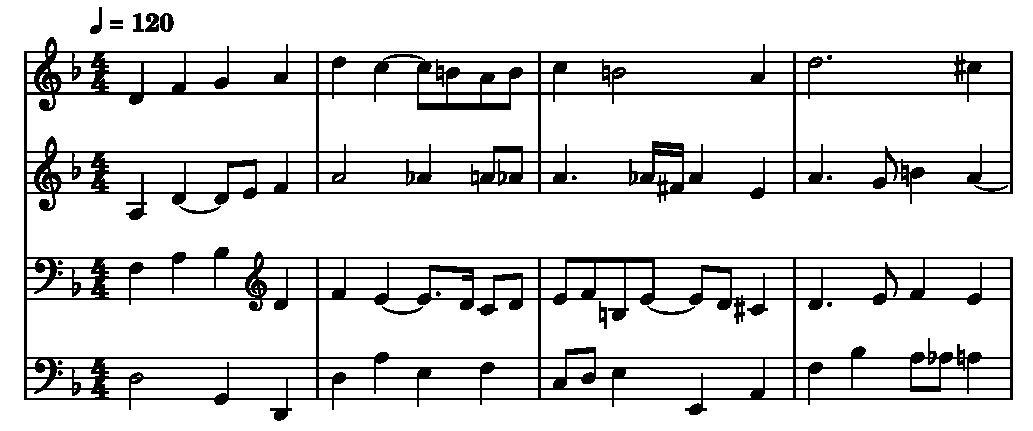
\includegraphics[width=0.9\linewidth]{./img/jsb_7_sheet.pdf}
    \end{center}
    \caption{Fragment chorału J.S. Bacha}\label{fig:jsb_sheet}
\end{figure}
\subsection{WAV i MP3}
WAV (ang. \textit{Waveform audio format}) jest binarnym zapisem plików, który jest znany z tego, że jest w stanie zapisywać dźwięk nie używając żadnego algorytmu kompresji. W związku z tym rozmiary tych plików są bardzo duże, co sprawia, że ich przechowywanie ich wymaga znacznego miejsca na dysku co może być problematyczne, kiedy zbiór danych jest bardzo duży. Plik WAV jest najrzetelniejszą cyfrową reprezentacją dźwięku analogowego. Tak duży rozmiar danych zawdzięcza się temu, że dźwięk jest zapisywany z częstotliwością 44.1 kHz, czyli 44100 sampli na sekundę. Format został stworzony w roku 1991 roku, jest jednym z najbardziej rozpowszechnionym formatów i jest obsługiwany przez praktycznie każde oprogramowanie edycji dźwięku. W celu wizualizacji dokonano syntezacji?? utworu przedstawionego w postaci nutowej na obrazku \ref*{fig:jsb_sheet} w związku z czym powstała fala dźwiękowa przedstawiona na grafice \ref*{fig:jsb_wav}.

\begin{figure}
    \begin{center}
        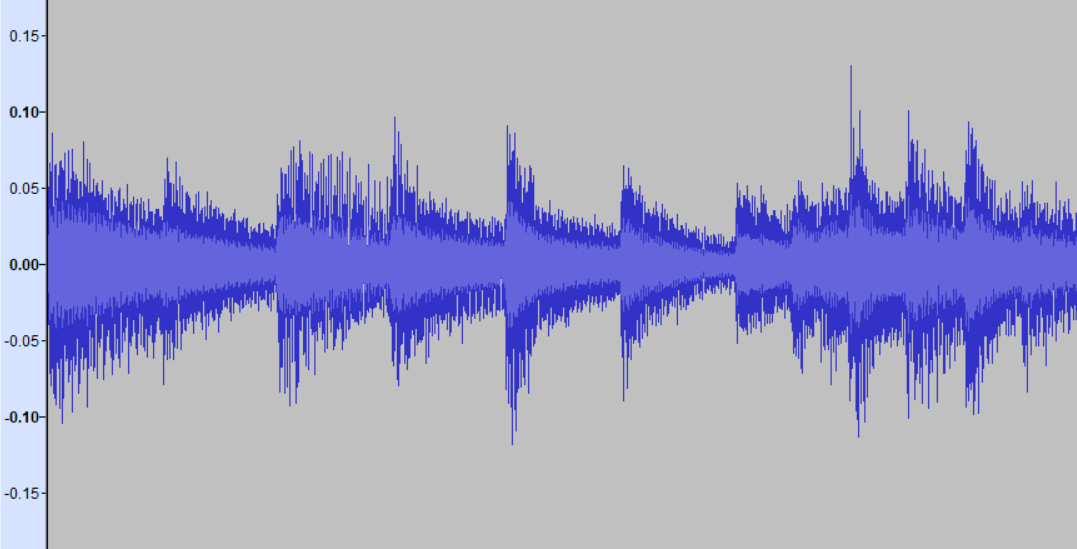
\includegraphics[width=\linewidth]{./img/jsb_wav.png}
    \end{center}
    \caption{Plik \textit{.wav} otworzony w programie Audacity.}\label{fig:jsb_wav}
\end{figure}

Często nie jest potrzebne przechowywanie bezstratne dźwięku, ponieważ i tak większość informacji, można zachować przy użyciu mniejszej ilości danych. Jednym z najpopularniejszych standardów kodowania stratnego jest MP3. Kompresja zmniejsza dokładność kodowania jak i również ``ucina" częstotliwości, które nie są słyszalne dla człowieka. Stratne kodowanie próbuje zachować równowagę pomiędzy jakością dźwięku a rozmiarem pliku. W kontekście uczenie maszynowego, zmniejszona ilość sampli przy zachowaniu większości informacji jest zjawiskiem pożądanym, ponieważ udaje nam się przynajmniej częściowo rozwiązać problem związany z ``przekleństwem wymiarowości".
\subsection{MIDI (ang. \textit{Musical Instrument Digital Interface})}
MIDI jest standardem, który opisuje protokół komunikacji, interfejs cyfrowy oraz złącze pozwalające połączyć ze sobą elektroniczne instrumenty, komputery oraz inne muzyczne peryferia. Pojedynczy kabel MIDI jest w stanie przekazać informacje na temat szesnastu na raz nadających kanałów z czego każdy może pochodzić z innego instrumentu. Każda interakcja z instrumentem, czyli przykładowo naciśnięty klawisz, szarpnięta struna, jest zapisana jako ``\textit{event}'', który zachowuje wartości takie jak konkretny znacznik czasu, wysokość dźwięku czy jego głośność. Dane pochodzące z urządzeń są zapisywane w specjalnym pliku, głównie o rozszerzeniu \textit{.mid} lub \textit{.midi}. Plik pozwala na przechowanie, rozpowszechnianie jak i również edycje dźwięków. W związku z tym, że w pliku nie jest przechowywany zapis konkretnej fali dźwiękowej zapisanej przez mikrofon, pozwala to na późniejszą zmianę np. instrumentu, który będzie odtwarzał zapisane dźwięki.

Typowym przedstawieniem zapisanych danych jest tak zwany \textit{piano roll}, który można porównać do dwuwymiarowego układy współrzędnych, gdzie wspołrzedna horyzontalna opisuje czas, a horyzontalna konkretne dźwięki pokazane jako klawisze pianina. Przykładowe porównanie zapisu MIDI z zapisem nutowym przedstawiono na grafice \ref*{fig:jsb_pianoroll} oraz \ref*{fig:jsb_sheet}.

\begin{figure}[ht!]
    \begin{center}
        \includegraphics*[width=\linewidth]{./img/piano_roll.png}
    \end{center}
    \caption{Muzyka zapisana w pliku MIDI}\label{fig:jsb_pianoroll}
\end{figure}

Warto zaobserwować, że zapis pliku w formacie MIDI umożliwia zdecydowanie większą ekspresje, ponieważ jest to zapis odtworzenia przez artystę pewnego utworu. Ten sposób nie ogranicza muzyki sztywno do konkretnego rytmu zdefiniowanego przez autora.

\subsection{Notacja ABC}
Notacja ABC jest systemem zapisywania nut w postaci czystego tekstu znakami ASCII. Notacja pojawiła sie w latach 70 XX wieku w celu zapisu i nauki tradycyjnych irlandzkich melodii, a nastepnie w kolejnej dekadzie została rozwinięta przez Chrisa Walshawa, który zapisywał w niej tradycyjne melodie zanim nauczył się standardowego zachodniego zapisu nutowego. Zapis ten posłużył do stworzonego przez niego programu \textit{abc2mtex}, który na podstawie notacji ABC generował komendy pozwalające zapis partytur w postaci \textit{MusicTex}. Obecnie używanym standardem jest wersja z roku 2011.

\begin{figure}[ht!]
    \begin{minted}{text}
X:1
T:Chorał no.7
A:J.S. Bach
Q:1/4=120
V:1
L:1/16
M:4/4
K:C clef=G2
D4F4G4A4|d4c6B2A2B2|c4B8A4|d12^c4|
V:2
L:1/16
M:4/4
K:C clef=G2
A,4D6E2F4|A8^G4A2^G2|A6^G^F^G4E4|A6G2B4A4|
V:3
F,4A,4^A,4D4|F4E7DC2D2|E2F2B,2E4D2^C4|D6E2F4E4|
V:4
L:1/16
M:4/4
K:C clef=F4
D,8G,,4D,,4|D,4A,4E,4F,4|C,2D,2E,4E,,4A,,4|F,4^A,4A,2^G,2A,4|        
\end{minted}
    \caption{Zapis wielu głosów w notacji ABC.}\label{abc:polyphony}
\end{figure}

Jak widać notacja ABC w dość zwięzły sposób zapisuje partyturę. Poza konkretnymi nutami oraz rytmem w tym formacie możemy zapisac również dodatkowe informacje na temat utworu. Każda linijka zaczynająca się się od znaku A-Z a następnie dwukropkiem jest tak zwanym ``polem informacyjnym". W tych polach zapisywac można takie informacje jak tytuł utworu lub metrum oraz wiele innych informacji między innymi dotyczące z jakiego zbioru muzycznego pochodzi dany utwór. Wiele z tych informacji powinna być usunięta w procesie preprocessingu danych, tak aby model dostał tylko te informacje, które rzeczywiście pomogą w nauce struktury muzyki. Do takich pól należy przede wszystkim domyślna długość nuty (L:), metrum (M:) oraz tonacja (K:) w jakiej utwór został napisany. Każda z tych informacji jest możliwa do "odgadnięcia" przez model, jednak podając modelowi te informację wyraźnie, mamy większą kontrolę nad procesem treningu. Dodatkową zaletą podawania tych informacji podczas treningu jest możliwość podania ich jako początkowa sekwencja na podstawie której model dalej będzie próbował kończyć melodię, przez co mamy kontrolę np. nad tym w jakiej tonacji i w jakim metrum zostanie wygenerowany nasz utwór.

Notacja ABC wpiera również melodie polifoniczne przy pomocy tagów V. Ich ilość nie jest ograniczona w związku z czym można w tym zapisie jest możliwe ujęcie nawet muzyki orkiestrowej. Dość skrajnym przykładem jest zapis drugiej części VII symfonii Ludwiga van Beethovena, która składa się aż z 19 instrumentów \cite{beethoven}.

\subsubsection{Tokenizacja plików MIDI}
Token jest odrębnym elementem, częścią sekwencji tokenów. W języku naturalnym tokenem może być znak, zaimek lub słowo. Zdanie może być następnie tokenizowane na sekwencję tokenów reprezentujących słowa i znaki interpunkcyjne. W przypadku muzyki tokeny mogą reprezentować wartości atrybutów nut (wysokość, wartość, czas trwania) lub zdarzenia czasowe. Token może przyjmować jedną z trzech form:
\begin{itemize}
    \item nazwa tokenu - słowna reprezentacja \textit{eventu} MIDI np. \textit{Pitch\_50}
    \item id - unikalna wartość liczbowa przypisana konkretnemu zdarzeniu
    \item bajt - unikalny bajt, który został przydzielony podczas treningu tokenizera
\end{itemize}

Słownictwo jest zapisywane w postaci \textit{look up table} łączącej nazwę tokenu z odpowiadającym jej id lub bajtem. Trening tokenizera polega na obliczeniu kodowania gramatykowego np. \textit{byte pair encoding} do postaci tabelarycznej w celu wykorzystania ich w dalszym modelowaniu.

Poza tokenami, które tokenizer tworzy na podstawie pliku MIDI dodaje on również dodatkowe takie jak:
\begin{itemize}
    \item PAD - token używany w przypadku kiedy w \textit{batchu} długość sekwencji jest różna; w takim przypadku tym tokenem wydłuża się sekwencje aby wszystkie miały długość najdłuższej
    \item BOS - token oznaczający początek sekwencji
    \item EOS - token oznaczający koniec sekwencji
\end{itemize}

Istnieje wiele algorytmów tokenizacji MIDI, jednak aby przedstawić mechanizm działania przyjrzymy?? się algorytmowi REMI. Revamped MIDI \cite{remi} reprezentuje nuty jako sekwencja tokenów wysokości tonu, mocy? i długości trwania oraz czas przy pomocy tokenu taktu oraz pozycji. Token taktu oznacza początek nowego taktu, a pozycji jego miejsce w obecnym takcie. Porównanie pomiędzy zapisem nutowym a jego reprezentacją można zaobserwować na grafice \ref*{fig:remi_notes} i \ref*{fig:remi_tokens}. Wiele algorytmów jest zaimplementowana w bibliotece MidiTok dla języka Python \cite{miditok2021}.

\begin{figure}
    \begin{center}
        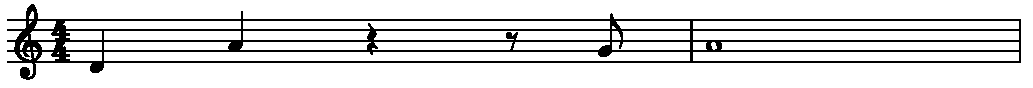
\includegraphics[width=0.9\linewidth]{./img/tokenizer_notes.pdf}
    \end{center}
    \caption{Prosta sekwencja muzyczna}\label{fig:remi_notes}
\end{figure}

\begin{figure}
    \begin{center}
        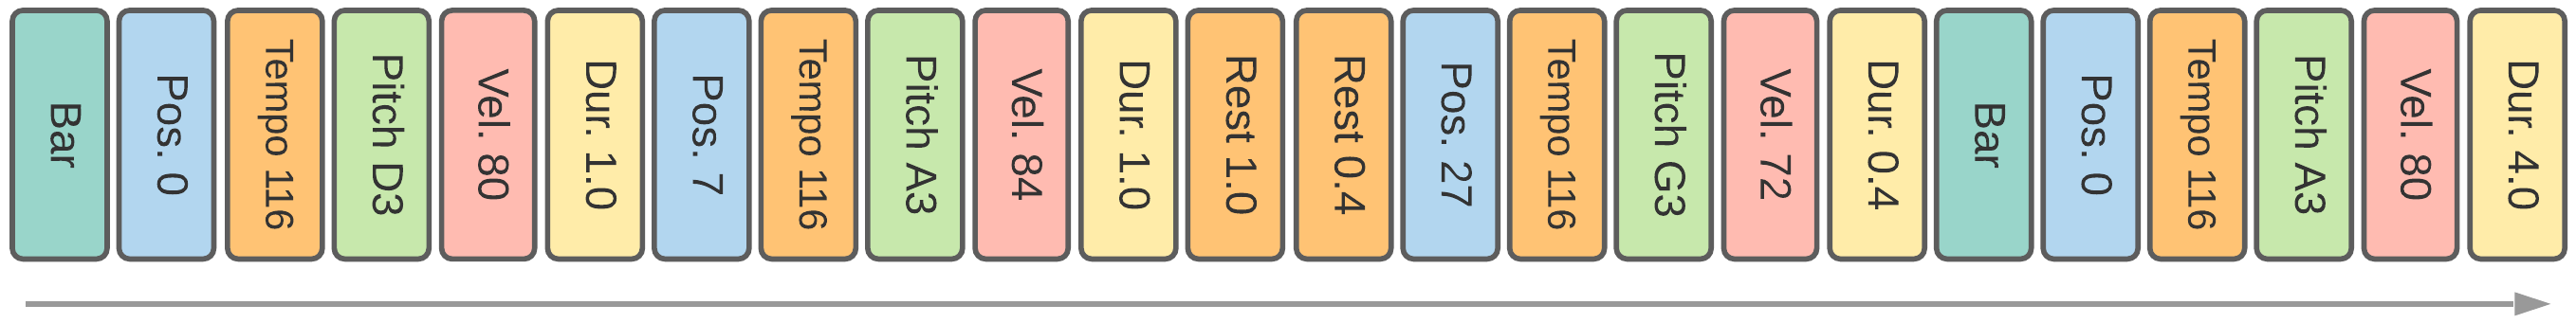
\includegraphics[width=0.9\linewidth]{./img/remi.png}
    \end{center}
    \caption{Reprezentacja muzyki w postaci tokenów}\label{fig:remi_tokens}
\end{figure}

\subsection{Porównanie zapisu muzycznego}

\begin{comment}
Tutaj na pewno opiszę 1. ile na dysku zajmują dane i 2. jaka jest długość sekwencji danych 3. Pros and cons jakiejś takie sensowne
\end{comment}

\section{Zbiory danych}

\subsection{Johann Sebastian Bach Chorales}
Dataset \cite{bachchorales}

\subsection{The MAESTRO v3.0}
Dataset \cite{maestrov3}

\subsection{Million Song Dataset}
Dataset i takie cytowanko \cite{milionsongs}

\section{STOA}
Tutaj nie wiem do końca w jakiej kolejności chciałbym o tym pisać, ponieważ z jednej strony przedstawienie STOA przed czymkolwiek jest ok, ale nie chciałbym pisać o czymś czego jeszcze w pracy nie wprowadziłem.

\section{Architekturze transformera}
\subsection{Algorytm uwagi (ang. \textit{attention})}
\subsection{Warianty mechanizmu uwagi}
\subsubsection{Self attention}
\subsubsection{Multi-headed attention}
\subsubsection{Flash attention}
\subsection{Budowa transformera}
\begin{figure}[!ht]
    \begin{center}
        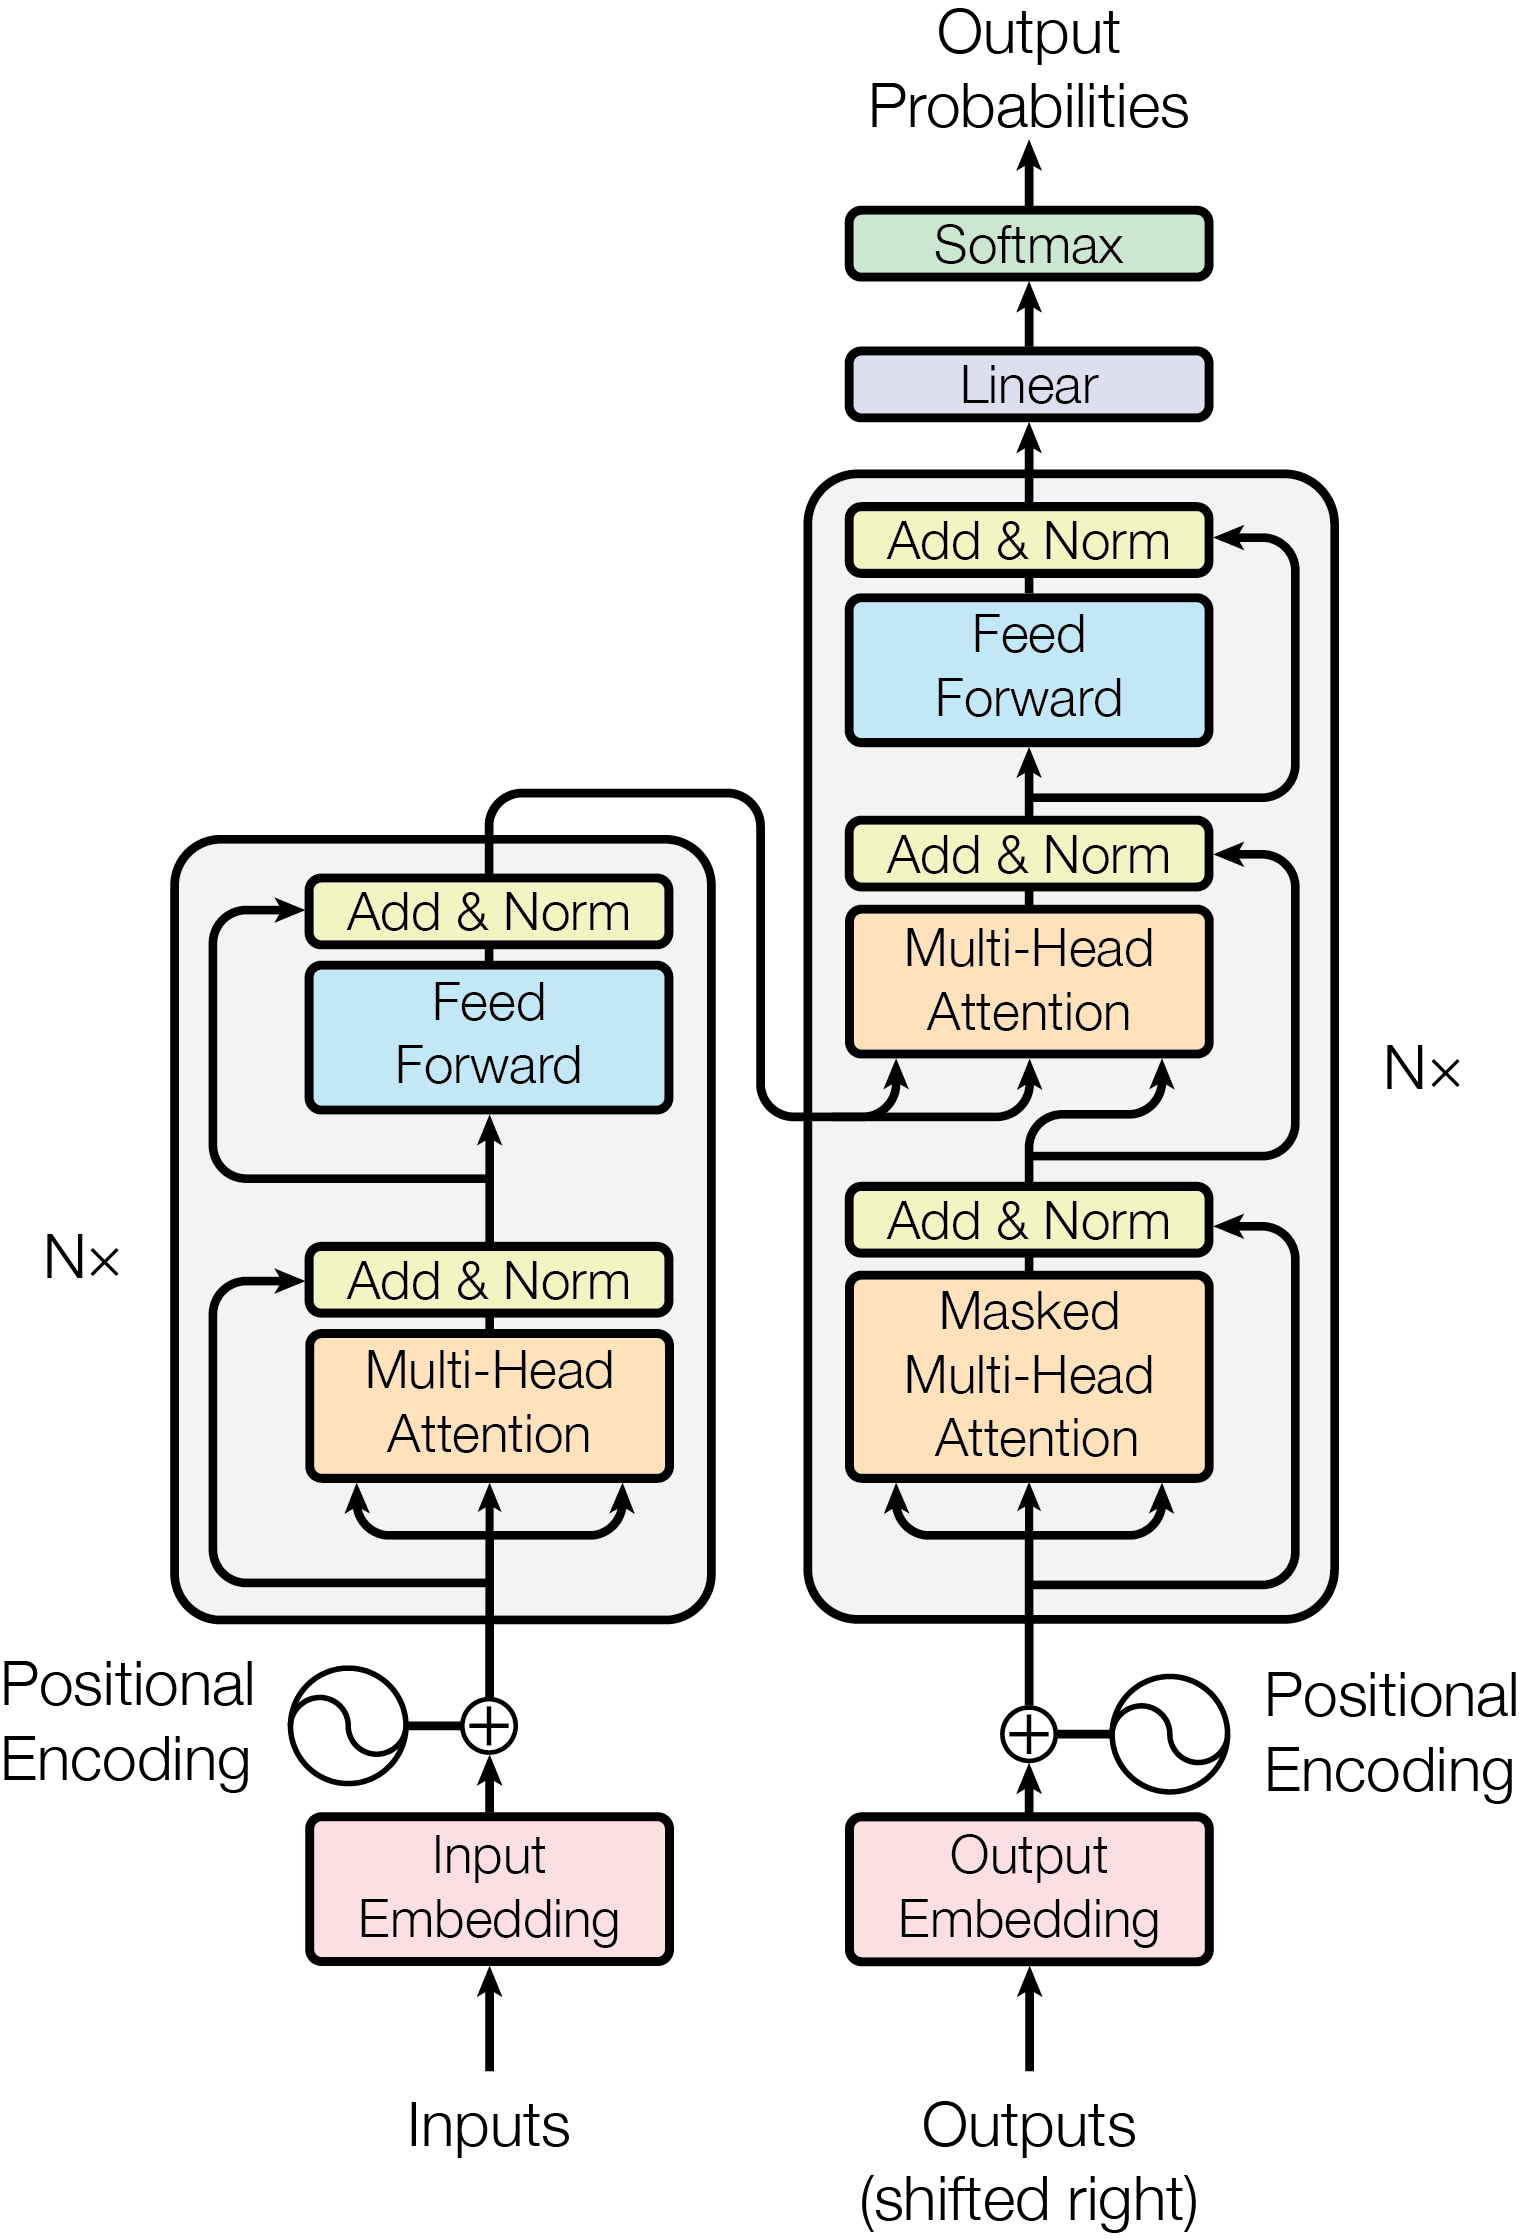
\includegraphics[width=0.7\linewidth]{img/transformer1}
    \end{center}
    \caption{Schemat transformera.}
    \label{fig:transformer1}
\end{figure}
\subsection{Modele tranformerowe}
\subsubsection{\textit{Classic} transformer}
\subsubsection{SeqGAN}
\subsubsection{Mistral}

\section{Architektura \textit{state space}}
\subsection{Mamba}
\subsection{Tutaj się rozdrobnić trzeba}
\begin{figure}
    \begin{center}
        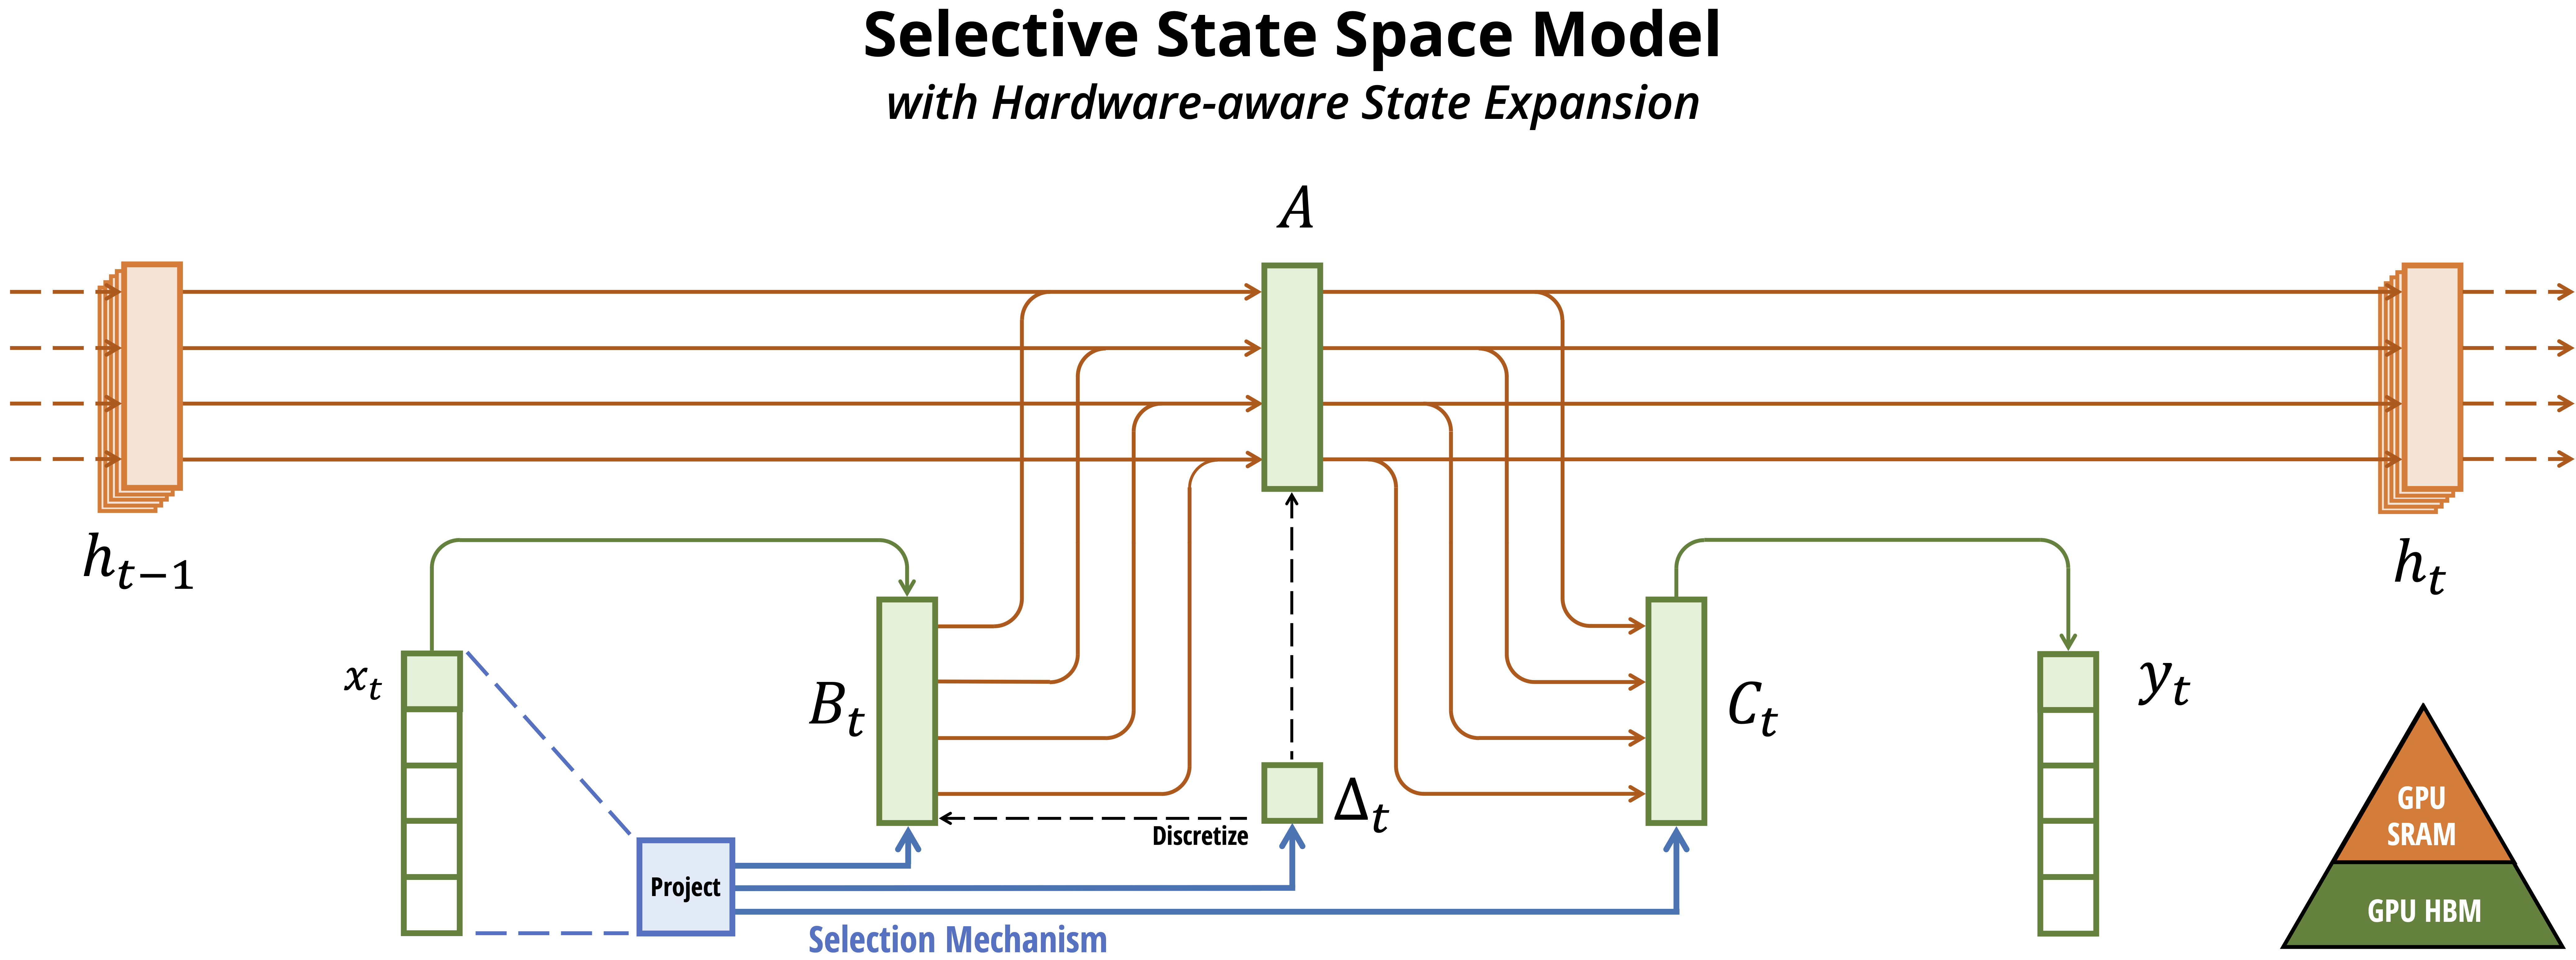
\includegraphics[width=0.9\linewidth]{img/mamba1.png}
    \end{center}
    \caption{Schemat modelu Mamba.}
    \label{fig:mamba1}
\end{figure}

\begin{comment}
Tytuł oraz strukturę rozdziału należy ustalić z opiekunem pracy.
\end{comment}

Aktualny stan wiedzy, na dany temat, na podstawie dostępnej literatury naukowej oraz specjalistycznej.
\chapter{Propozycja rozwiązania}
\chapter{Przeprowadzenie eksperymentów}
\begin{comment}
Tytuł oraz strukturę rozdziału należy ustalić z opiekunem pracy.
\end{comment}
\section{Opis \textit{pipeline-u}}
Tutaj zamierzam opisać w jaki sposób modele zostały stworzone, jakie bilbioteki zostały użyte, jaki sprzęto został użyty podczas treningu
\section{Porównanie architektur użytych modeli}
\section{Prezentacja otrzymanych wyników}
\section{Porównanie wyników}
Celem porównania otrzymanych wyników z dowolnych modeli, jest ocena jakości ich pracy. W kontekście modeli dyskryminujących (ang. \textit{discriminative model}), na przykład klasyfikatorów bądź modeli regresyjnych, ocena ich jakości jest dość prosta, ponieważ istnieje predefiniowana, prawdziwa wartość w zbiorze testowym, którą model próbuje przewidzieć. W takim przypadku ewaluacja jakości modelu to porównanie prawdziwych danych, z tymi przewidzianymi przez model. Porównanie odbywa się przez policzenie metryk np. dla modelu klasyfikującego celności, precyzji, \textit{F1-score} lub dla modelu regresyjnego MSE lub $R^2$. W przypadku modeli generacyjnych celem treningu jest jak najlepsza aproksymacja rozkładu prawdopodobieństwa danych $P(X_{data})$ lub w przypadku danych oznaczonych łączny rozkład $P(X, Y)$. W przypadku dużej wymiarowości danych, obliczenie obiektywnych metryk takich jak \textit{log-likelihood} lub dywergencja Kullbacka-Leiblera (\textit{KLD}) często jest nieobliczalne. Dla człowieka weryfikacja wyników modeli generacyjnych takich jak \textit{text-to-speech} lub \textit{text-to-image} jest trywialnym zadaniem, jednak nie jest to oczywiste zadanie algorytmiczne. Często odwołuje się do subiektywnych metryk takich jak \textit{MOS ang. mean opinion score}, które oblicza się jako średnią opinię np. w skali od 1-5 braną z zazwyczaj niewielkiej grupy ludzi. Niestety metryka ta często nie jest wiarygodna ze względu na jej subiektywności niewielką próbę badawczą. Aby wyeliminować te wady serwisy takie jak \textit{HuggingFace} udostępniają narzędzia dla członków społeczności, które pozwalają na ranking modeli, z nadzieją że zgodnie z prawem wielkich liczb, przy wystarczającej liczbie odpowiedzi, uda się otrzymać w miarę obiektywną ocenę. Przykładowym narzędziem tego rodzaju jest \textit{The TTS Arena}\cite{tts_arena}, która pozwala na ranking modeli \textit{text-to-speech}.

W przypadku muzyki, istnieje możliwość aby zweryfikować poprawność wygenerowanych sekwencji odwołując się do teorii oraz harmonii muzyki. Istnieje kilka narzędzi takich jak \textit{Chordify}, \textit{Hooktheory} lub \textit{Sibelius}, które pozwalają na analizę harmoniczną utworów, dzieki czemu autorzy mogą w prosty sposób analizować i dobierać progresję danej melodii. Niestety większość takich narzędzi jest płatna i nie pozwala na zautomatyzowaną analizę wielu plików. Dodatkowym problemem jest w analizie harmonicznej, szczególnie prowadzonej przez algorytmy, jest rozróżnienie harmonii wertykalnej oraz horyzontalnej. Rozróżnienie to zostało wytłumaczone przez Jacoba Colliera, kilkukrotnego laureata nagród \textit{Grammy}, którego zdaniem akord, który nawet zagrany sam brzmi niepoprawnie, w odpowiednim kontekście i przez odpowiednią progresję w kolejnych fragmentach muzyki, może mieć nadany sens, przez co cała sekwencja nabiera muzycznego piękna\cite{collier_wrongnote}.
\begin{comment}
W mojej pracy prawdopodobnie zostanie zastosowane podejście MOS dla dość niewielkiej grupy ludzi, jednak jeśli triale oprogramowania pozwola, spróbuję przynajmniej sprawdzić czy taka analiza pozwala na jakieś sensowne obliczenie metryki
\end{comment}
Brak obiektywnych metryk, którymi można się posłużyć podczas ewaluacji modelu jest dodatkowym problemem w momencie \textit{fine-tunigu} modelu. Ciężko jest wybrać odpowiednie rozwiązanie architektoniczne lub odpowiednie hiperparametry, kiedy jedyną miarą jakości wygenerowanych danych jest subiektywna opinia programisty lub grupy osób wybranych jako wyrocznia.
\chapter{Zakończenie}
\begin{comment}
Tytuł oraz strukturę rozdziału należy ustalić z opiekunem pracy.
\end{comment}
\begin{enumerate}
    \item Podsumowanie.
    \item Możliwości dalszego rozwoju.
    \item Potencjalne obszary zastosowania pracy.
\end{enumerate}
%%%%%%%%%%%%%%%%%%%%%%%%%%%%%%%%%%%%%
%%%%%%%%%%%%%%%%%%%%%%%%%%%%%%%%%%%%%
\appendix % Dodatek
\chapter{Typowe elementy składowe pracy dyplomowej z informatyki}
\section{Tabele}
\begin{comment}
\begin{itemize}
    \item Każda tabela powinna być opisana w treści pracy.
    \item Podpis ma być przed tabelą.
\end{itemize}
\end{comment}
W tabeli \ref{tab:result} przedstawiono wyniki pomiarów.
\begin{table}[!h]
    \caption{Pomiary zużycia energii elektrycznej\label{tab:result}.}
    \centering
    \begin{tabular}{|l||r@{,}l|}
        \hline
        \textbf{L.p.} & \multicolumn{2}{|c|}{\textbf{Wartość}}          \\
        \hline
        \hline
        \cline{2-3}
        %\textbf{L.p.} & \multicolumn{1}{r@{\,\vline\,}}{Całkowita} & Ułamkowa \\
        \hline
        1             & 12345                                  & 6789   \\
        \cline{2-3}
                      & 45                                     & 89     \\
        \hline
        2             & 45                                     & 678901 \\
        \hline
    \end{tabular}
\end{table}

Jeżeli tabela zawiera dużą liczbę wierszy i może nie zmieścić się na stronie \pauza patrz tabela \ref{tab:longtable} \pauza skorzystaj z pakietu \emph{longtable} \cite{longtable}.
\begin{longtable}{|p{14ex}|p{1.5em}|p{1.5em}|p{1.5em}|p{1.5em}|p{1.5em}|p{1.5em}|p{1.5em}|p{1.5em}|p{1.5em}|}
    \caption{Tabela, która zawiera dużą liczbę wierszy\label{tab:longtable}.}
    \endfirsthead
    \hline
              & 1 & 2 & 3 & 4 & 5 & 6 & 7 & 8 & \\
    \cline{2-9}
              &   &   &   &   &   &   &   &   & \\
    \hline
    \endhead
    \endfoot
    \hline\hline
              & 1 & 2 & 3 & 4 & 5 & 6 & 7 & 8 & \\
    \cline{2-9}
              &   &   &   &   &   &   &   &   & \\
    \hline\hline
    Student 1 &   &   &   &   &   &   &   &   & \\
    \cline{2-9}
              &   &   &   &   &   &   &   &   & \\
    \hline\hline
    Student 2 &   &   &   &   &   &   &   &   & \\
    \cline{2-9}
              &   &   &   &   &   &   &   &   & \\
    \hline\hline
    Student 3 &   &   &   &   &   &   &   &   & \\
    \cline{2-9}
              &   &   &   &   &   &   &   &   & \\
    \hline\hline
    Student 4 &   &   &   &   &   &   &   &   & \\
    \cline{2-9}
              &   &   &   &   &   &   &   &   & \\
    \hline\hline
    Student 5 &   &   &   &   &   &   &   &   & \\
    \cline{2-9}
              &   &   &   &   &   &   &   &   & \\
    \hline\hline
    Student 6 &   &   &   &   &   &   &   &   & \\
    \cline{2-9}
              &   &   &   &   &   &   &   &   & \\
    \hline\hline
    Student 7 &   &   &   &   &   &   &   &   & \\
    \cline{2-9}
              &   &   &   &   &   &   &   &   & \\
    \hline\hline
    Student 8 &   &   &   &   &   &   &   &   & \\
    \cline{2-9}
              &   &   &   &   &   &   &   &   & \\
    \hline\hline
    Student 9 &   &   &   &   &   &   &   &   & \\
    \cline{2-9}
              &   &   &   &   &   &   &   &   & \\
    \hline\hline
    % Student 10 &   &   &   &   &   &   &   &   & \\
    % \cline{2-9}
    %            &   &   &   &   &   &   &   &   & \\
    % \hline\hline
    % Student 11 &   &   &   &   &   &   &   &   & \\
    % \cline{2-9}
    %            &   &   &   &   &   &   &   &   & \\
    % \hline\hline
    % Student 12 &   &   &   &   &   &   &   &   & \\
    % \cline{2-9}
    %            &   &   &   &   &   &   &   &   & \\
    % \hline\hline
    % Student 13 &   &   &   &   &   &   &   &   & \\
    % \cline{2-9}
    %            &   &   &   &   &   &   &   &   & \\
    % \hline\hline
\end{longtable}

Tabele, w których występuje długi tekst, a co za tym idzie może się on nie zmieścić \pauza musi zostać zawinięty, z pomocą przychodzi środowisko 'tabularx' \cite{tabularx} \pauza  patrz tabela \ref{tab:tabularx}.
\begin{table}[!ht]
    \caption{Tabela zawierająca długi tekst\label{tab:tabularx}.}
    \centering
    \begin{tabularx}{300pt}{|c|X|c|X|}
        \hline
        \multicolumn{2}{|c|}{Wpis wielokolumnowy!} &
        TRZY                                       &
        CZTERY                                       \\
        \hline
        jeden                                      &
        \raggedright\arraybackslash Szerokość tej kolumny zależy od
        szerokości tabeli.                         &
        trzy                                       &
        \raggedright\arraybackslash Kolumna czwarta będzie zachowywać się w taki sam sposób jak
        druga kolumna o tej samej szerokości.        \\
        \hline
    \end{tabularx}
\end{table}
%%%%%%%%%%%%%%%%%%%%%%%%%%%%%%%%%%%%%
\section{Rysunki}
\begin{comment}
\begin{itemize}
    \item Rysunki powinny być przerysowane samodzielnie albo używane tylko te,
          których twórcy zezwolili na ich rozpowszechnianie oraz kopiowanie, czyli
          np. rysunki objęte licencją Creative Commons.
    \item Każdy rysunek powinien być opisany w treści pracy.
\end{itemize}
\end{comment}
\subsection{Wewnętrzne}
Klasa \emph{agh-wi}, automatycznie, dołącza pakiet \emph{TikZ} \cite{tikz} \pauza dostarcza on komend pozwalających na tworzenie grafik. Przykładowe grafiki pokazano na rysunku \ref{fig:tikz1} oraz \ref{fig:tikz2}.
%%%%%%%%%%%%%%%%%
\begin{figure}[!h]
    \begin{center}
        \tikz \draw[thick,rounded corners=8pt]
        (0,0) -- (0,2) -- (1,3.25) -- (2,2) -- (2,0) -- (0,2) -- (2,2) -- (0,0) -- (2,0);
    \end{center}
    \caption{Prosty rysunek \emph{TikZ}\label{fig:tikz1}.}
\end{figure}
%%%%%%%%%%%%%%%%%
\begin{figure}[!ht]
    \begin{center}
        \begin{tikzpicture}
            \draw[step=.5cm,gray,very thin] (-1.4,-1.4) grid (1.4,1.4);
            \draw (-1.5,0) -- (1.5,0);
            \draw (0,-1.5) -- (0,1.5);
            \draw (0,0) circle [radius=1cm];
        \end{tikzpicture}
    \end{center}
    \caption{Bardziej złożony rysunek \emph{TikZ}\label{fig:tikz2}.}
\end{figure}
%%%%%%%%%%%%%%%%%

Oprócz rysunków eksponowanych możliwe jest tworzenie grafik będących  \tikz{\fill[orange] (0ex,0ex) circle (1ex);  \fill[red] (1ex,1ex) circle (1ex);} częścią \tikz{\draw (0pt,0pt) -- (20pt,6pt);} zdania.

\emph{TikZ} pozwala również na kreślenie po powierzchni strony, np. możemy narysować strzałki pomiędzy elementami strony.
\begin{shaded}
    %%%%%%%%%%%%%%%%%%%%%%%%%%%%%%%%%%%%%%%%%%%%%%%%%%%
    % Zmodyfikowana wersja przykładu ze strony  https://texample.net/tikz/examples/global-nodes/
    %%%%%%%%%%%%%%%%%%%%%%%%%%%%%%%%%%%%%%%%%%%%%%%%%%%
    Ułamek \pauza patrz wzór \ref{eqn:tikz} \pauza składa się z:
    \begin{itemize}
        \item Licznika \tikz[na] \node (n1) {};
    \end{itemize}
    %%%%%%%%%%%%%%%%%
    \begin{equation}
        a =  \frac{\tikz[baseline] \node[fill=blue!20,rectangle] (t1){$x+y$};}{\tikz[baseline] \node[fill=red!20, ellipse] (t2){$y-z$}; }
        \label{eqn:tikz}
    \end{equation}
    %%%%%%%%%%%%%%%%%
    \begin{itemize}
        \item Mianownika \tikz\node[na] (n2) {};
    \end{itemize}
    %%%%%%%%%%%%%%%%%
    \begin{tikzpicture}[overlay]
        \path  (n1) edge [->,bend left] (t1);
        \path  (n2) edge [->,bend right] (t2);
    \end{tikzpicture}
\end{shaded}
\subsection{Zewnętrzne}
Oczywiście możliwe jest również dołączanie rysunków zewnętrznych \pauza
pakiet \emph{graphicx} \cite{graphicx} pozwala na wstawianie grafik zapisanych w  plikach: '.png', '.jpg' oraz '.pdf'. Rysunek \ref{fig:logo} wstawiono przy użyciu tego pakietu.
\begin{figure}[!ht]
    \begin{center}
        \IfFileExists{img/logo_podstawowe.png}{
            
\includegraphics[width=0.7\linewidth]{img/logo_podstawowe}
        }
        {Nie znaleziono pliku 'img/logo\_podstawowe.png' \pauza pobierz go ze strony \url{https://www.informatyka.agh.edu.pl/media/uploads/Logo WI/PNG/logo_podstawowe.png}}
    \end{center}
    \caption{Logo Wydziału Informatyki.}
    \label{fig:logo}
\end{figure}
%%%%%%%%%%%%%%%%%%%%%%%%%%%%%%%%%%%%%
\section{Kody źródłowe}
Najpopularniejszymi pakietami, które umożliwiają składanie kodów źródłowych programów, są:
\begin{description}
    \item[listings \cite{listings}] \pauza kod źródłowy jest formatowany bezpośrednio przez \LaTeX{}\dywiz{}a \pauza nie jest używany żaden, zewnętrzny, formater kodu.
        \begin{lstlisting}[language=C++, float=ht, label=lst:code1, caption={Przykładowy kod źródłowy sformatowany za pomocą pakietu 'listings'.}]
/* Pierwszy program w C++ */

#include <iostream>

int main() {
std::cout << "Hello World!";
return 0;
}
\end{lstlisting}
    \item[minted \cite{minted}] \pauza formatuje kod źródłowy przy użyciu biblioteki języka Python  o nazwie \emph{Pygments} \cite{pygments}.
        \begin{listing}[!ht]
            \caption{Przykładowy listing sformatowany za pomocą pakietu 'minted'.\label{lst:code2}}
            \begin{minted}{c++}
/* Pierwszy program w C++ */

#include <iostream>

int main() {
std::cout << "Hello World!";
return 0;
}
\end{minted}
        \end{listing}
\end{description}

\begin{comment}
\begin{itemize}
    \item Podpis ma być przed kodem źródłowym.
    \item \alert{Proszę używać tylko jednego z tych pakietów}; w przeciwnym razie otrzymasz taki efekt, jak w przykładowej pracy \pauza obydwa listingi mają ten sam numer.
\end{itemize}
\end{comment}

Kod źródłowy w C++ sformatowany przy użyciu pakietu \emph{listings}, pokazano na listingu \ref{lst:code1}; sformatowany przy użyciu pakietu \emph{minted}, pokazano na listingu \ref{lst:code2}.
%%%%%%%%%%%%%%%%%%%%%%%%%%%%%%%%%%%%%
\section{Algorytmy}
Pakiet \emph{algorithm2e} \cite{algorithm2e} to jeden z kilku, które pozwalają zapisywać algorytmy w formie pseudokodu \pauza patrz
algorytm \ref{alg:algo_disjdecomp}.
\begin{comment}
Podpis ma być przed algorytmem.
\end{comment}
\begin{algorithm}[!htb]
    \caption{Disjoint decomposition.}\label{alg:algo_disjdecomp}
    %%%%%%%%%%%%%%%%%%%%%%%%%%     
    \SetKwData{Left}{left}\SetKwData{This}{this}\SetKwData{Up}{up}
    \SetKwFunction{Union}{Union}\SetKwFunction{FindCompress}{FindCompress}
    \SetKwInOut{Input}{input}\SetKwInOut{Output}{output}
    \Input{A bitmap $Im$ of size $w\times l$}
    \Output{A partition of the bitmap}
    \BlankLine
    \emph{special treatment of the first line}\;
    \For{$i\leftarrow 2$ \KwTo $l$}{
        \emph{special treatment of the first element of line $i$}\;
        \For{$j\leftarrow 2$ \KwTo $w$}{\label{forins}
            \Left$\leftarrow$ \FindCompress{$Im[i,j-1]$}\;
            \Up$\leftarrow$ \FindCompress{$Im[i-1,]$}\;
            \This$\leftarrow$ \FindCompress{$Im[i,j]$}\;
            \If(\tcp*[h]{O(\Left,\This)==1}){\Left compatible with \This}{\label{lt}
                \lIf{\Left $<$ \This}{\Union{\Left,\This}}
                \lElse{\Union{\This,\Left}}
            }
            \If(\tcp*[f]{O(\Up,\This)==1}){\Up compatible with \This}{\label{ut}
                \lIf{\Up $<$ \This}{\Union{\Up,\This}}
                \tcp{\This is put under \Up to keep tree as flat as possible}\label{cmt}
                \lElse{\Union{\This,\Up}}\tcp*[h]{\This linked to \Up}\label{lelse}
            }
        }
        \lForEach{element $e$ of the line $i$}{\FindCompress{p}}
    }
\end{algorithm}\DecMargin{1em}
%%%%%%%%%%%%%%%%%%%%%%%%%%%%%%%%%%%%%
\section{Wzory}
\LaTeX{} bardzo dobrze sprawdza się w przypadku prac dyplomowych zawierających wzory matematyczne\footnote{ W przypadku złożonych wzorów warto zastosować pakiet \emph{amsmath} \cite{amsmath}.}.
\subsection{Przykłady}
Wzór $E = mc^{2}$\nomenclature{$c$}{Prędkość światła w próżni} jest częścią zdania.

\begin{equation}
    \left|\sum_{i=1}^n a_ib_i\right|
    \le
    \left(\sum_{i=1}^n a_i^2\right)^{1/2}
    \left(\sum_{i=1}^n b_i^2\right)^{1/2}
\end{equation}

% Do wstawienia poniższych wzorów użyto środowisk (otoczeń) zdefiniowanych w pakiecie 'amsmath'
Wartości zmiennej opisano wzorem \ref{eq:r1}.
\begin{equation}
    \label{eq:r1}
    x=\begin{cases}
        y           & \text{dla } y > 0    \\
        \frac{z}{y} & \text{dla } y \leq 0
    \end{cases}
\end{equation}

Wzór \ref{eq:r2} to wzór wielowierszowy.
\begin{align}
    \label{eq:r2}
    2x^2 + 3(x-1)(x-2) & =2x^2 + 3(x^2-3x+2)             \\
                       & = 2x^2 + 3x^2 - 9x + 6\nonumber \\
                       & = 5x^2 - 9x + 6\nonumber
\end{align}
\begin{comment}
Należy używać tylko dwóch rodzajów wzorów:
\begin{enumerate}
    \item \enquote{W linii}.
    \item Eksponowane, numerowane.
\end{enumerate}
\end{comment}
%%%%%%%%%%%%%%%%%%%%%%%%%%%%%%%%%%%%%
\section{Twierdzenia i podobne struktury}
Twierdzenie nr \ref{tw} opublikował, w roku 1691, francuski matematyk Michel Rolle.
\begin{theorem}[Rolle'a]
    \label{tw}
    Jeśli dana funkcja f: $\mathbb R \to \mathbb R$ jest:
    \begin{enumerate}
        \item ciągła w przedziale $[a,b]$
        \item jest różniczkowalna w przedziale $(a,b)$
        \item na końcach przedziału $[a,b]$ przyjmuje równe wartości: $f(a) = f(b)$,
    \end{enumerate}
    to w przedziale $(a,b)$ istnieje co najmniej jeden punkt c taki, że $f'(c) = 0$.
\end{theorem}

Teraz coś z informatyki \ldots
\begin{definition}
    Bit to najmniejsza jednostka informacji w komputerze.
\end{definition}
\begin{definition}
    Bajtem nazywamy ciąg ośmiu bitów.
\end{definition}
%%%%%%%%%%%%%%%%%%%%%%%%%%%%%%%%%%%%%
\backmatter % Część końcowa
%%%%%%%%%%%%%%%%%%%%%%%%%%%%%%%%%%%%%
\chapter{Uwagi Autora}
\begin{itemize}
    \item Aktualna wersja klasy jest dostępna pod adresem \url{https://github.com/polaksta/LaTeX/tree/master/agh-wi}\footnote{W przypadku Overleaf-a jest ona pod adresem  \url{https://www.overleaf.com/read/fnvcvqjyrbyw\#5ac622}}.
    \item Skoro Twoja praca dyplomowa powstała w \LaTeX{}u, to zachęcam Cię również do przygotowania prezentacji (na obronę pracy magisterskiej) w tym języku. Najpopularniejszą klasą do tworzenia tego typu dokumentów jest \emph{beamer} \cite{beamer}.
    \item Pod adresem \url{https://github.com/polaksta/LaTeX/tree/master/beamerthemeAGH}\footnote{W przypadku Overleaf-a jest on pod adresem  \url{https://www.overleaf.com/read/fkjdthnbrfhj\#9c6184}} możesz znaleźć, stworzony przeze mnie,  nasz uczelniany szablon dla prezentacji \LaTeX{} Beamer.
    \item Treść wszystkich rozdziałów tej, przykładowej, pracy dyplomowej znajduje się w jednym pliku \pauza \textbf{nie jest to polecane rozwiązanie}. W przypadku pisania własnej pracy warto umieścić zawartość każdego z rozdziałów w osobnych plikach, a następnie dołączać je do dokumentu głównego \pauza patrz opis na stronie \url{https://www.dickimaw-books.com/latex/thesis/html/include.html}.
    \item Jeżeli pewne elementy mają być wyróżniane w \alert{jednakowy} \alert{sposób}, to proponuję nie używać bezpośredniego stylowania, tzn.
          \mint{tex}{\colorbox{red!50}{jednakowy} \colorbox{red!50}{sposób}} ale zdefiniować własną komendę stylującą, np. \verb+\alert+,
          \mint{tex}{\newcommand{\alert}[1]{\colorbox{red!50}{#1}}}
          a następnie użyć jej w dokumencie.
          \mint{tex}{\alert{jednakowy} \alert{sposób}}

          Dzięki temu, jeżeli będziesz chciał / chciała zmienić sposób stylowania tych elementów, np. niebieskie tło zamiast czerwonego, to wystarczy zmodyfikować, tylko, definicję komendy, zamiast zastępować, w tekście pracy dyplomowej, wybrane (niekoniecznie wszystkie!) wystąpienia tekstu \texttt{red}, tekstem \texttt{blue}.
\end{itemize}
Stanisław Polak

%%%%%%%%%%%%%%%%%%%%%%%%%%%%%%%%%%%%%
%%%%%%%%%%%%%%%%%%%%%%%%%%%%%%%%%%%%%
% Wyświetl spis literatury
% UWAGA: Powinien zawierać tylko te publikacje, do których odwołujesz się w pracy
\printbibliography
%%%%%%%%%%%%%%%%%%%%%%%%%%%%%%%%%%%%%
%%%%%%%%%%%%%%%%%%%%%%%%%%%%%%%%%%%%%
\end{document}